% arara: pdflatex: { synctex: yes }
% arara: makeindex: { style: ctuthesis }
% arara: bibtex

% The class takes all the key=value arguments that \ctusetup does,
% and a couple more: draft and oneside
\documentclass[twoside]{ctuthesis}

\ctusetup{
	preprint = \ctuverlog,
	mainlanguage = english,
	titlelanguage = english,
%	mainlanguage = czech,
	otherlanguages = {slovak,english},
	title-czech = {Moje bakalářka se strašně, ale hrozně dlouhým předlouhým názvem},
	title-english = {Drone detection using neural networks from combined RGB camera and LiDAR data},
	subtitle-czech = {Cesta do tajů kdovíčeho},
%	subtitle-english = {Journey to the who-knows-what wondeland},
	doctype = B,
	faculty = F3,
	department-czech = {Katedra matematiky},
	department-english = {Department of Cybernetics},
	author = {Adam Škuta},
	supervisor = {Matouš Vrba},
	supervisor-address = {Ústav X, \\ Uliční 5, \\ Praha 99},
	supervisor-specialist = {Martin Saska},
	fieldofstudy-english = {Mathematical Engineering},
	subfieldofstudy-english = {Mathematical Modelling},
	fieldofstudy-czech = {Matematcké inženýrství},
	subfieldofstudy-czech = {Matematické modelování},
	keywords-czech = {slovo, klíč},
	keywords-english = {word, key},
	day = 10,
	month = 2,
	year = 2017,
	specification-file = {ctutest-zadani.pdf},
%	front-specification = true,
%	front-list-of-figures = false,
%	front-list-of-tables = false,
%	monochrome = true,
%	layout-short = true,
}

\ctuprocess

\addto\ctucaptionsczech{%
	\def\supervisorname{Vedoucí}%
	\def\subfieldofstudyname{Studijní program}%
}

\ctutemplateset{maketitle twocolumn default}{
	\begin{twocolumnfrontmatterpage}
		\ctutemplate{twocolumn.thanks}
		\ctutemplate{twocolumn.declaration}
		\ctutemplate{twocolumn.abstract.in.titlelanguage}
		\ctutemplate{twocolumn.abstract.in.secondlanguage}
		\ctutemplate{twocolumn.tableofcontents}
		\ctutemplate{twocolumn.listoffigures}
	\end{twocolumnfrontmatterpage}
}

% Theorem declarations, this is the reasonable default, anybody can do what they wish.
% If you prefer theorems in italics rather than slanted, use \theoremstyle{plainit}
\theoremstyle{plain}
\newtheorem{theorem}{Theorem}[chapter]
\newtheorem{corollary}[theorem]{Corollary}
\newtheorem{lemma}[theorem]{Lemma}
\newtheorem{proposition}[theorem]{Proposition}

\theoremstyle{definition}
\newtheorem{definition}[theorem]{Definition}
\newtheorem{example}[theorem]{Example}
\newtheorem{conjecture}[theorem]{Conjecture}

\theoremstyle{note}
\newtheorem*{remark*}{Remark}
\newtheorem{remark}[theorem]{Remark}

\setlength{\parskip}{5ex plus 0.2ex minus 0.2ex}
\graphicspath{{figures/}}

% Abstract in Czech
\begin{abstract-czech}
\end{abstract-czech}

% Abstract in English
\begin{abstract-english}
\end{abstract-english}

% Acknowledgements / Podekovani
\begin{thanks}
Děkuji ČVUT, že mi je tak dobrou \emph{alma mater}.
\end{thanks}

% Declaration / Prohlaseni
\begin{declaration}
Prohlašuji, že jsem předloženou práci vypracoval samostatně, a že jsem uvedl veškerou použitou literaturu.

V Praze, \ctufield{day}.~\monthinlanguage{title}~\ctufield{year}
\end{declaration}

% Only for testing purposes
\listfiles
\usepackage[pagewise]{lineno}
\usepackage{lipsum,blindtext}
\usepackage{mathrsfs} % provides \mathscr used in the ridiculous examples
\usepackage{todonotes}
\usepackage{amsmath}
\usepackage{xspace}
\usepackage{caption}
\usepackage{subcaption}
\usepackage{multirow}

\begin{document}

\maketitle
\chapter{Introduction}
The goal of this thesis was to prove whether a usage of LiDAR data coupled with images from RGB was useful for the localization of UAVs in contrast to the usage of image data alone. The LiDAR and RGB camera was be mounted on top of the scanner UAV. All the measurements were taken inside a virtual environment, with a realistic UAV and sensor simulation. The dataset was then be preprocessed and used as the input to a Convolutional neural network for the object detection. The preprocessing was as following:
\begin{itemize}
	\item Coordinate transformation for the non-matching coordinate systems,
	\item Projection of 3d points into a 2d image,
	\item Using a Convolutional neural network or other postprocessing methods to generate more points in a sparse LiDAR pointcloud,
	\item Fusing RGB images and dense LiDAR data into RGBD images.
\end{itemize}
These data were then used as a training and validation dataset for drone detection convolutional neural network. Different approaches in terms of preprocessing RGBD images were utilized and compared with the other state-of-the-art techniques used in this field.
\begin{figure}[h]
	\centering
	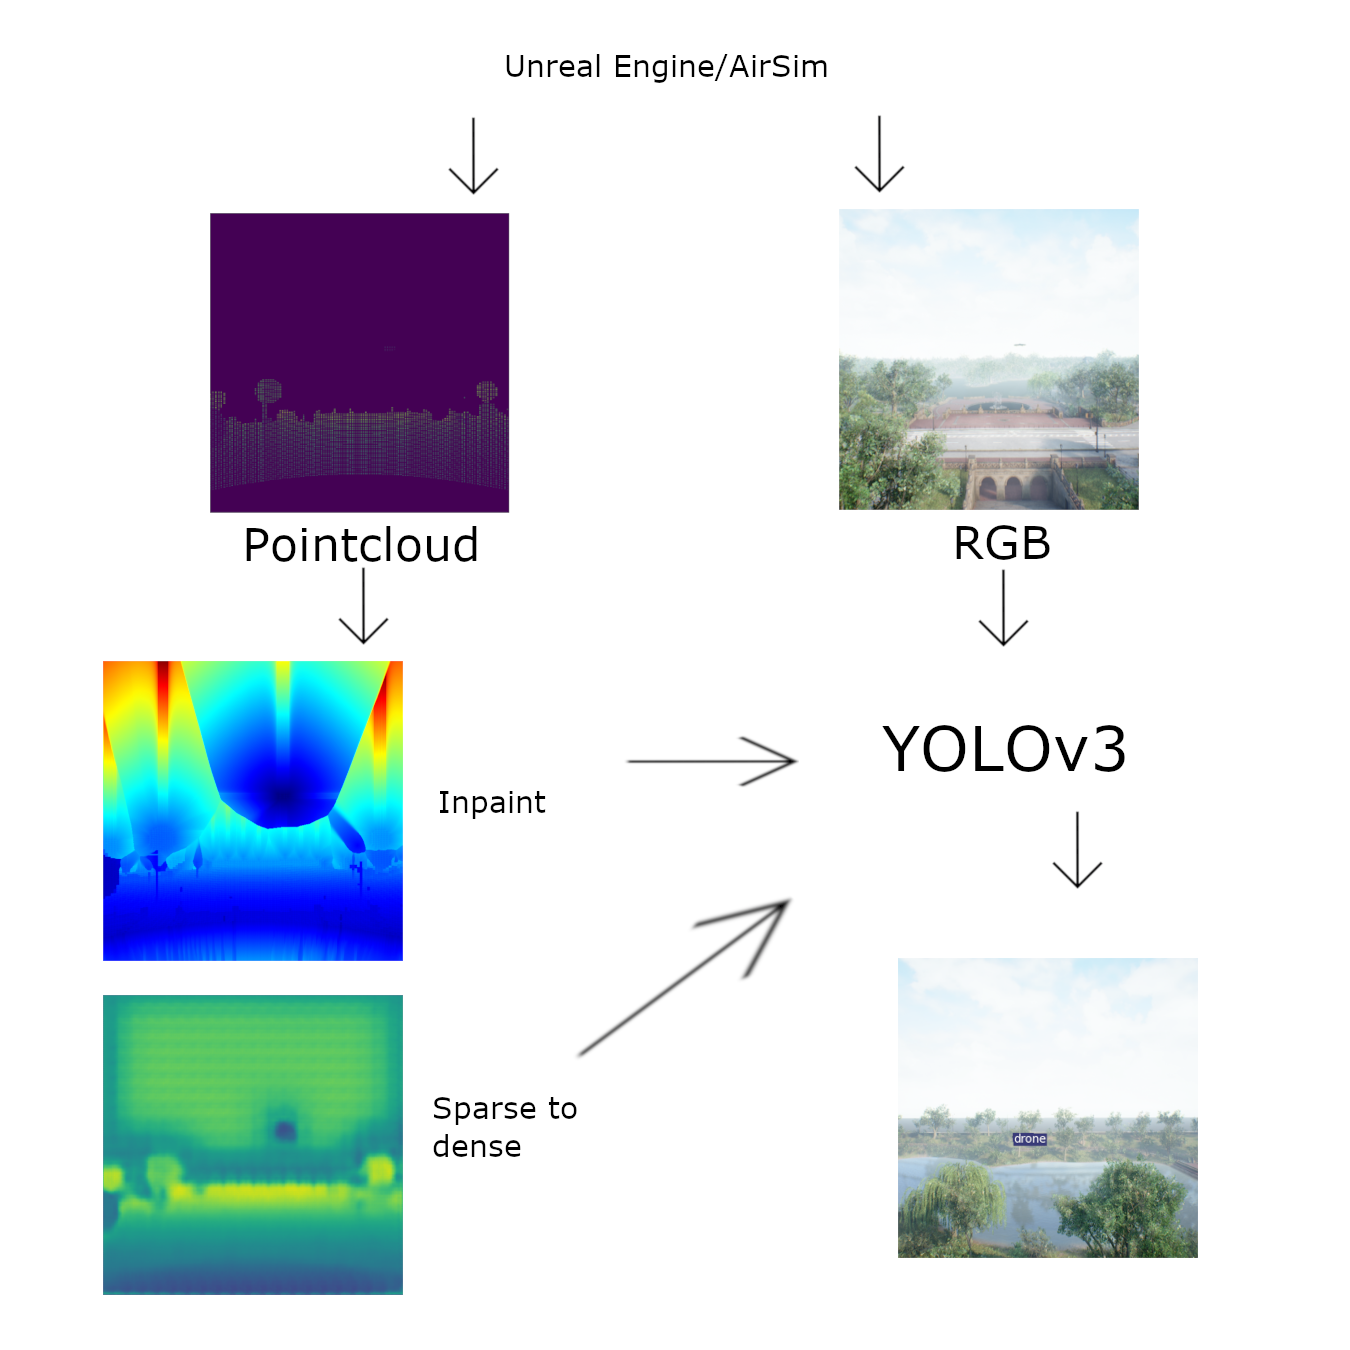
\includegraphics[width=\textwidth]{intro_schema.png}
	\caption{Schema of the process.}
\end{figure}
\pagebreak
\section{State of the art}
Drone detection is required for tracking and interception of other possibly misused drones. Most of the state-of-the-art techniques for drone detection are utilizing convolutional neural networks as a backbone for detection. They differ from each other mainly in the network architecture as well as types of input data. \newline
\newline
Expandable YOLO is modified convolutional network based on YOLOv3 architecture. It uses Darknet53 backbone and expands the detection heads to the third dimension as well as applies 3D Intersection over Union. The input is RGBD images taken from camera and RealSense depth camera. The network aims to simplify the network architecture for increase in processing speed.\\
\\
YOLO3D is a convolutional neural network that is based on YOLOv2 architecture, modifying its loss function with addition of yaw angle and 3D bounding boxes. The input consists of RGB images and birds eye pointcloud grid maps taken from LiDAR. The results show real-time performance on KITTI dataset.\\
\\
YOLOv5 is fifth iteration of the YOLO convolutional neural network architecture. The network provides different sizes based on the complexity of its task. Unlike its predecessors it is written entirely using PyTorch framework. 
\chapter{Convolutional neural networks}
A convolutional neural network was used in two problems in the thesis. First one was used on a sparse LiDAR pointcloud generating more points and therefore making it more dense. Second one was used for object, in this case drone, detection using RGB and RGBD data as the input.
\section{Sparse to dense}
Sparse to dense is a Convolutional neural network written in PyTorch. It predicts the depth measurements from sparse depth dataset. The size of the network is modifiable and can be chosen as training parameters.
\begin{figure}[h!]
	\caption{Example of different network architectures available.}
	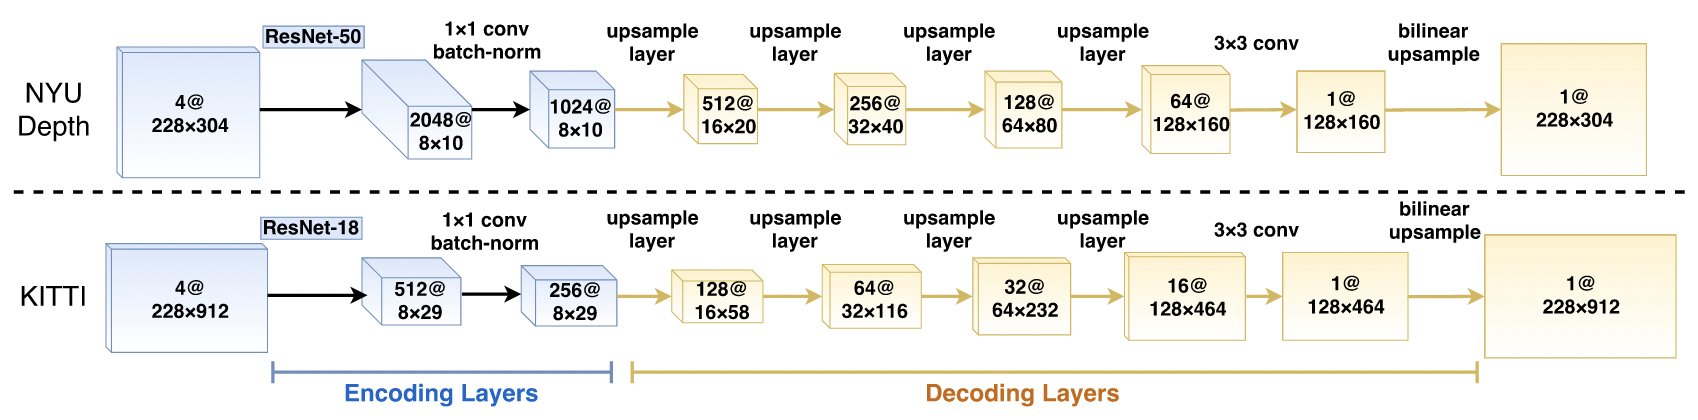
\includegraphics[width=\textwidth]{sparse2dense.png}
	\centering
\end{figure}\\
For the encoding and therefore input layers a ResNet-50 or ResNet-18 can be chosen, depending on the size of the input image for memory constraints. The decoding layers consist of 4 upsampling layers and a deconvolutional layer with either stride 2 or 3 or uprojection layer or upconvolutional layer as a choice for training. The default loss function is least absolute deviations also known as $L_1$ error:
\begin{equation}
	L_1=\sum_{i=1}^{n}|y_{true}-y_{predicted}|,
\end{equation}
where:
\begin{itemize}
	\item n is batch size,
	\item $y_{true}$ are real depth values,
	\item $y_{predicted}$ are predicted depth values.
\end{itemize}
The input to the network are RGBD images and the output is a depth map with the same dimensions as input. The depth input $D$ is sampled from the ground truth depth map $D^*$ with the following formula:
\begin{equation}
	D(i,j)=\begin{cases}
		D^*(i,j),&\text{with probability}\ p,\\
		0,&\text{otherwise},
	\end{cases}
\end{equation}
where:
\begin{itemize}
	\item $i,j$ are coordinates of the input image,
	\item $p=\frac{m}{n}$, where $m$ number of depth samples to be chosen at the start of training and $n$ is the total amount of available depth samples.
\end{itemize}
During training several input data augmentations take place. These augmentations include:
\begin{itemize}
	\item Scaling the input image by a random number $s\in[1,1.5]$,
	\item Rotating the input image by a random degree $r\in[-5,5]$,
	\item Scaling the brightness, contrast and saturation of the RGB component of the image by a random number $k\in[0.6,1.4]$,
	\item Normalizing the RGB component of the image,
	\item Flipping the image horizontally with a 50\% chance.
\end{itemize}
The output of the network is a dense depth image with the dimensions of the input. Every pixel contains predicted depth measurement in meters. The output of the Sparse to Dense network will be used for further training later.
\section{YOLOv3}
\todo{citations}
You only look once (YOLO) is a convolutional neural network model used mainly for object detection and recognition. The main advantage is its simplicity in comparison to similar convolutional neural networks, resulting in faster detection speeds. It belongs to the state of the art convolutional neural networks for object detection and recognition. The version used in this work is the third version YOLOv3. The backbone called Darknet53 consists of 53 convolutional layers. The original detector consists of 3 detection heads each responsible for detecting objects of various sizes.
\begin{figure}[h]
	\caption{YOLOv3 network architecture.}
	\centering
	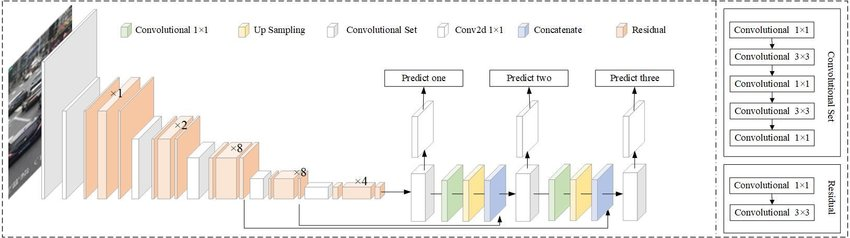
\includegraphics[width=\textwidth]{yolov3model.jpg}
\end{figure}
YOLOv3 takes $n$-channel images as the input and outputs are as following:
\begin{itemize}
	\item Offsets of the bounding box centers relative to the size of input image,
	\item Scales of the bounding boxes relative to their respective anchors,
	\item Objectness score, which dictates the confidence of object detection in the particular cell,
	\item Class score, which dictates the confidence of object recognition in the particular cell for each of the classes used during training.
\end{itemize}
The loss function used during the training is sum squared error loss or $L_2$ error described as follows:
\begin{equation}
	L_2=\sum_{i=1}^{n}(y_{true}-y_{predicted})^2,
\end{equation}
where:
\begin{itemize}
	\item $n$ is batch size,
	\item $y_{true}$ are ground truth bounding box values,
	\item $y_{predicted}$ are predicted bounding box values.
\end{itemize}
\section{Image inpainting method based on the Fast Marching Method} \label{inpainting}
Image inpainting is a method used for reconstructing missing values in the image. A one such method based on \todo{Citation} called Image inpainting method based in the Fast Marching Method is presented in this section. A grayscale image is used for simplification purposes.\\
\\
The grayscale value of a pixel to be inpainted is determined by the known neighboring pixel values. To compute grayscale value from one close pixel a following formula is used:
\begin{equation} \label{eq:1}
	I_q(p)=I(q)+\nabla I(q)(p-q),
\end{equation}
where:
\begin{itemize}
	\item $q$ is a pixel with known grayscale value,
	\item $p$ is a pixel with unknown grayscale value,
	\item $I(x)$ is a grayscale value at pixel $x$,
	\item $\nabla I(x)$ is a gradient value at pixel $x$.
\end{itemize}
To get a final value for the unknown pixel a Equation \ref{eq:1} is applied on all known pixels in a specified region $B_{\varepsilon}(p)$ from the unknown pixel. The function is as following:
\begin{equation}
	I(p)=\frac{\sum_{q\in B_{\varepsilon}(p)}w(p,q)I_q(p)}{\sum_{q\in B_{\varepsilon}(p)}w(p,q)},
\end{equation}
where $w(p,q)$ is a weighting function designed for propagating sharpness of the image.\\
\begin{figure}[h!]
	\caption{Example of the inpainting technique.}
	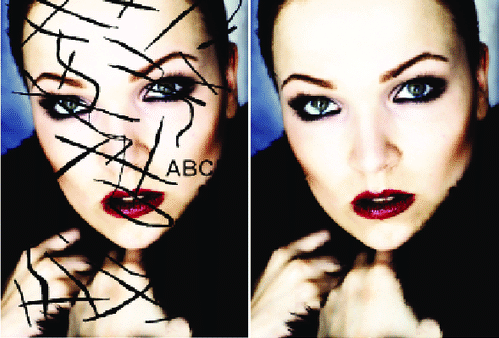
\includegraphics[width=\textwidth]{inpaint_example.png}
	\centering
\end{figure}\\
\chapter{Sensors}
\section{Coordinate systems}
In order to correctly label the data for training, a position of the second drone in relation to the camera mounted on the first one is required. The API call in AirSim returns a position in relation to its starting point. Therefore a transformation from the starting point of the second drone to the camera mounted on the first one is required. This transformation is written as follows:
\begin{equation}
	\textbf{T}=\textbf{T}_{d1}^{c}\textbf{T}_{s1}^{d1}\textbf{T}_{s2}^{s1},
\end{equation}
where:
\begin{itemize}
	\item $\textbf{T}_{s2}^{s1}$ is transformation from the starting point of the second drone to the starting point of the first drone,
	\item $\textbf{T}_{s1}^{d1}$ is transformation from the starting point of the first drone to the body of the first drone,
	\item $\textbf{T}_{d1}^{c}$ is transformation from the body of the first drone to the cameras coordinate system.
\end{itemize}
Transformation matrix $\textbf{T}$ is generally be described as follows:
\begin{equation}
	\textbf{T}=\begin{bmatrix}
		\textbf{R} & \textbf{p}\\
		\textbf{0}^T & 1
	\end{bmatrix},
\end{equation}
where:
\begin{itemize}
	\item $\textbf{R}$ is a 3x3 rotation matrix,
	\item $\textbf{p}$ is a 3x1 translation column vector,
	\item $\textbf{0}^T$ is a 1x3 row vector of zeros.
\end{itemize}
\section{Camera Model}
For the creation of the bounding boxes used for training and for processing raw data from LiDAR sensor a transformation from coordinate system of the camera to the pixel values of the image needs to be defined. For this task a pinhole camera model is used.
\begin{figure}[h]
	\centering
	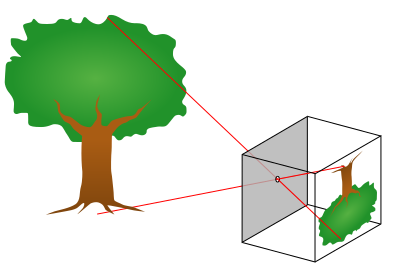
\includegraphics[width=\textwidth]{pinhole.png}
	\caption{Pinhole camera model.}
\end{figure}\\
The transformation is then defined as follows:
\begin{equation} \label{eq:2}
	\begin{bmatrix}
		x'\\
		y'
	\end{bmatrix}=
	\begin{bmatrix}
		f\frac{x}{z}+c_x\\
		f\frac{y}{z}+c_y
	\end{bmatrix},
\end{equation}
where:
\begin{itemize}
	\item $x'$ and $y'$ are pixel coordinate values on the image,
	\item $x$,$y$,$z$ are coordinate values of a point to be transformed,
	\item $f$ is focal length of the camera,
	\item $c_x$,$c_y$ are offsets on the image plane.
\end{itemize}
\chapter{Dataset}
The dataset for this work can be generated in two ways. The first is real-life drone shots mixed with point clouds from LiDAR mounted on top of a drone. The second is generating a dataset using a realistic virtual environment where a drone, camera and LiDAR are being emulated very close to their real-life counterparts. An advantage to this approach is that a great variety of environments can be chosen a lot of them often inaccessible otherwise (power plant, airport, snowy mountains out of season etc.). Therefore this approach was chosen for the task.
\section{Unreal Engine}
Unreal Engine is a software tool used for creating realistic 3d environments, most often used as a video game engine.
\todo{citation https://www.unrealengine.com/en-US/features} 
It is written in C++ and open-source supporting a variety of pre-built environments and assets. For this work three diferent environments were used for the creation of the dataset:
\begin{itemize}
	\item City Park Environment Collection,
	\item Automotive Winter Scene,
	\item Downtown West Modular Pack.
\end{itemize}
\pagebreak
\begin{figure}[h]
	\centering
	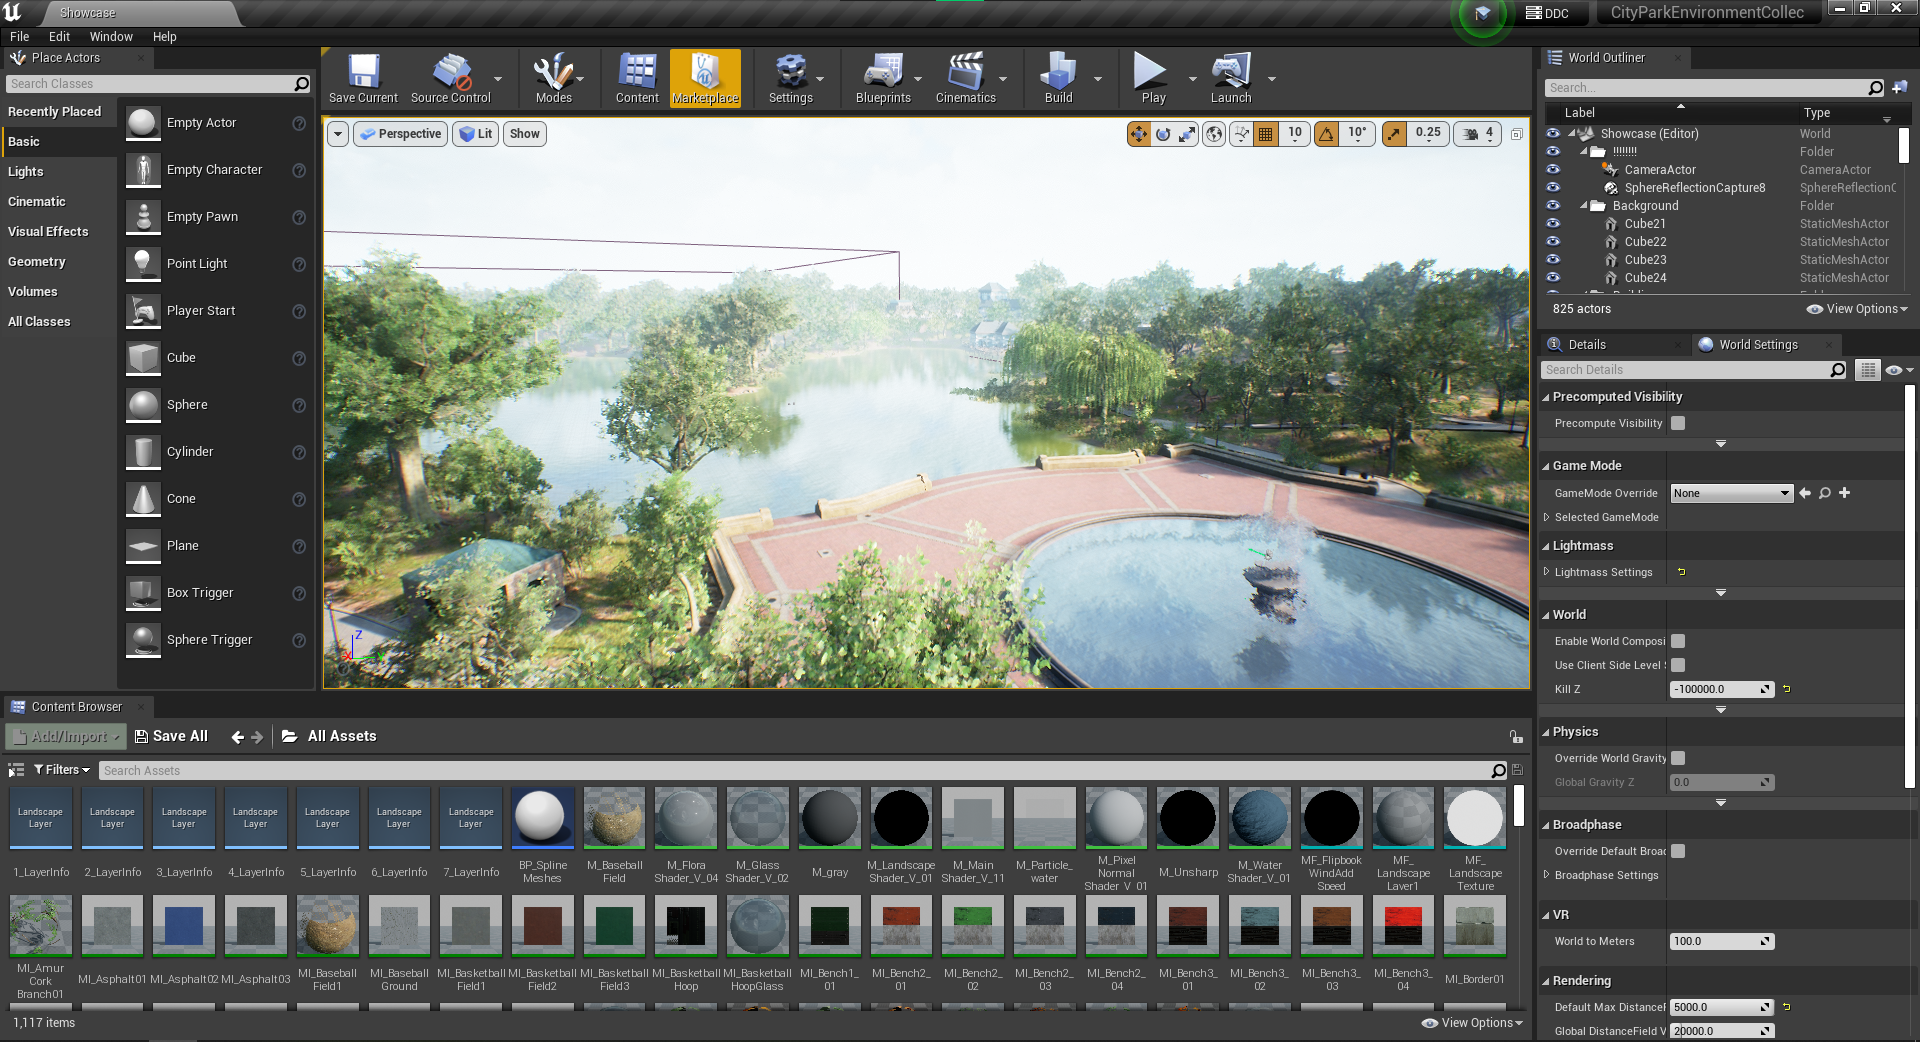
\includegraphics[width=\textwidth]{unreal_ui.png}
	\caption{Unreal Engine user interface.}
\end{figure}
Together 5320 pictures and labels were generated using two drones. One drone was equipped with RGB camera and LiDAR sensor and was responsible for taking the pictures and pointclouds from LiDAR. The second one was used as a model for drone detection.
\section{AirSim}
Open-source plugin for Unreal Engine called AirSim was used for the generation of the dataset. It simulates realistic flight motions of drones as well as seven types of sensors \todo{airsim zdroj}, including RGB camera and LiDAR used for this task. AirSim supports both a C++ API as well as Python API, latter which was used for controlling the motion and capturing the dataset. Location of the second drone was generated through API call, which produces a location of the drone in global coordinate system of the map, which is later transformed to the local coordinates of the first drone carrying the LiDAR and RGB sensors using Equation \ref{eq:2}. The capturing drone traveled on each map on a 3D cube grid.
\begin{figure}
	\centering
	\begin{subfigure}[b]{0.3\textwidth}
		\centering
		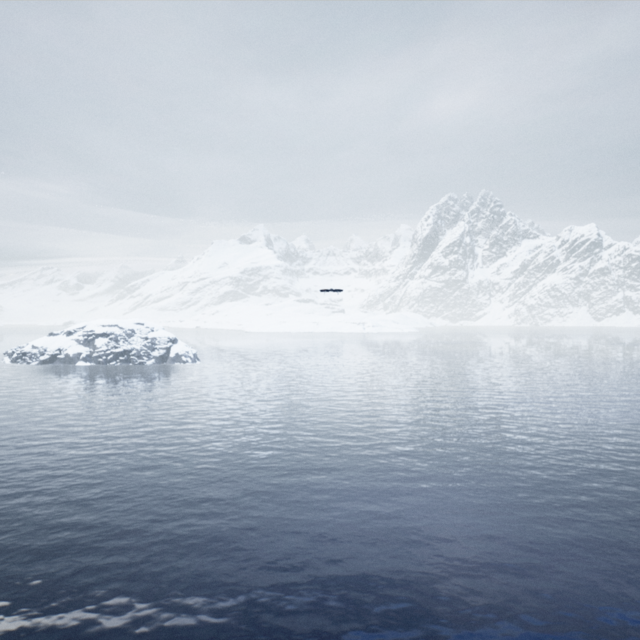
\includegraphics[width=\textwidth]{snow_rgb.png}
		\caption{Snow Environment.}
	\end{subfigure}
	\hfill
	\begin{subfigure}[b]{0.3\textwidth}
		\centering
		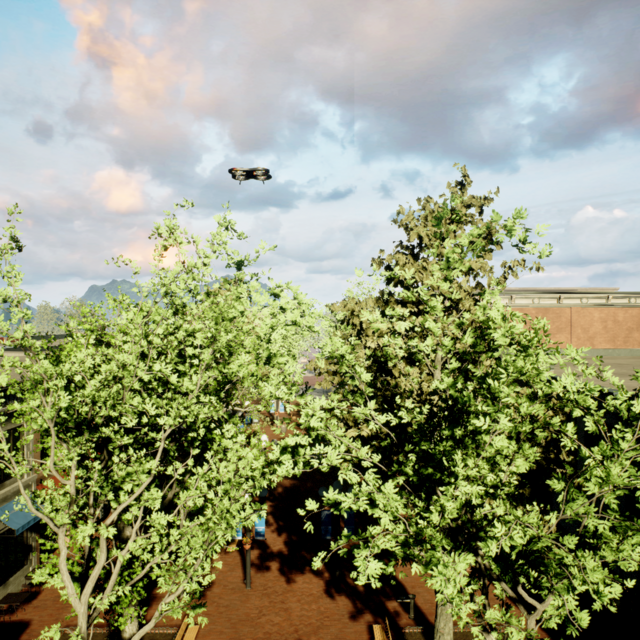
\includegraphics[width=\textwidth]{city_rgb.png}
		\caption{City Environment.}
	\end{subfigure}
	\hfill
	\begin{subfigure}[b]{0.3\textwidth}
		\centering
		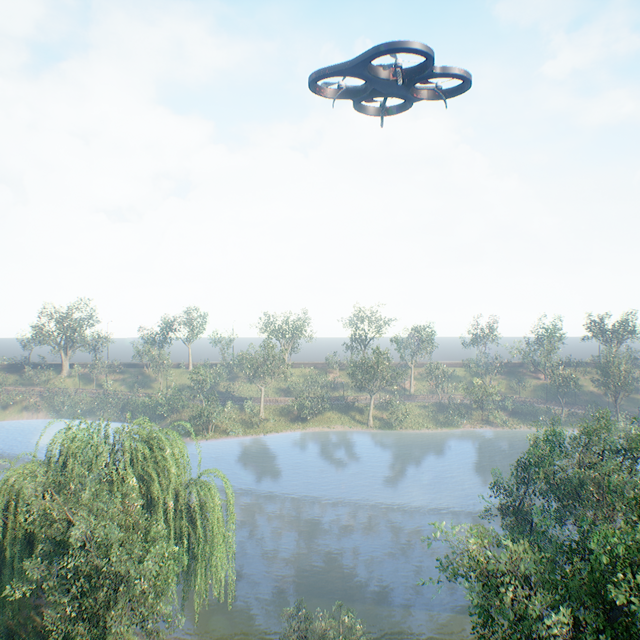
\includegraphics[width=\textwidth]{park_rgb.png}
		\caption{Park Environment.}
	\end{subfigure}
	\caption{Sample photos from each environment.}
\end{figure}
\chapter{Training}
For the training purposes 5320 samples were taken using AirSim simulator. Each sample consists of:
\begin{itemize}
	\item 640x640 3-channel RGB image from the camera,
	\item 640x640 1-channel sparse depth image from the LiDAR sensor,
	\item Label file containing ground truth bounding boxes values.
\end{itemize}
This dataset was split 90\% training samples to 10\% validation samples. 
\section{Sparse to Dense}
The data were trained using Sparse to Dense neural network to receive dense depth image. The training was done for 15 epochs using batch size of 8. The backbone was Resnet18 and decoder was set to Deconv3. The network was pretrained on Kitti dataset.
\begin{figure}
	\centering
	\begin{subfigure}[b]{0.4\textwidth}
		\centering
		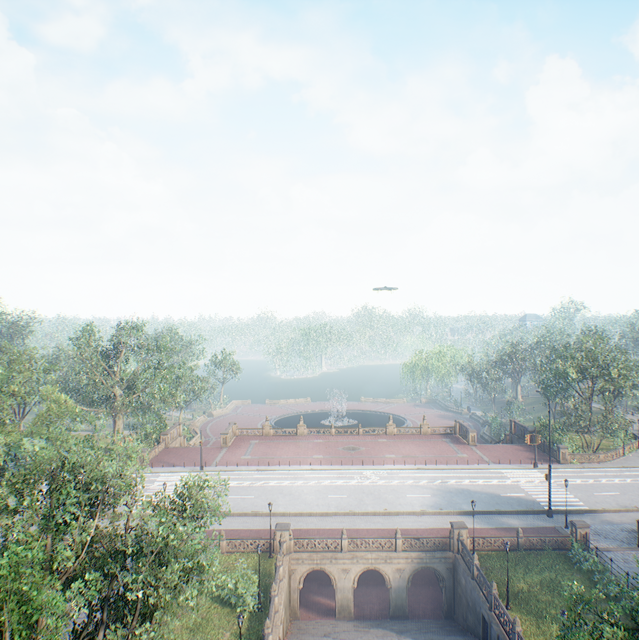
\includegraphics[width=\textwidth]{s2d_input.png}
		\caption{Input image.}
	\end{subfigure}
	\hfill
	\begin{subfigure}[b]{0.4\textwidth}
		\centering
		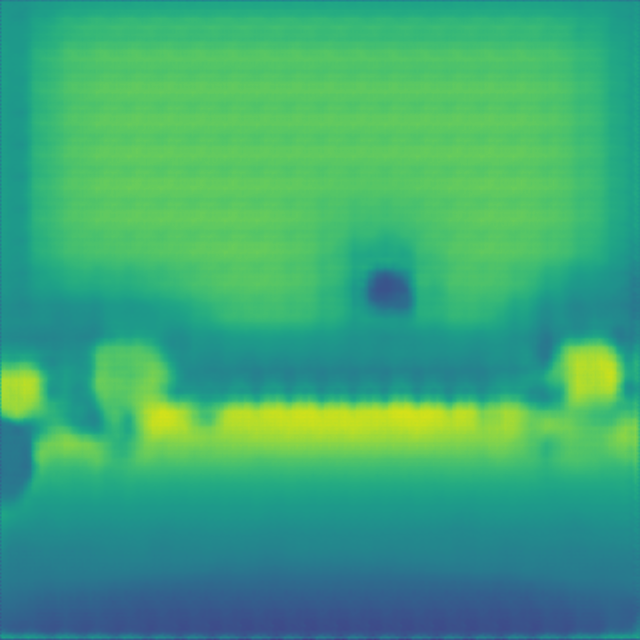
\includegraphics[width=\textwidth]{s2d_output.png}
		\caption{Output depth map.}
	\end{subfigure}
	\hfill
	\begin{subfigure}[b]{0.4\textwidth}
		\centering
		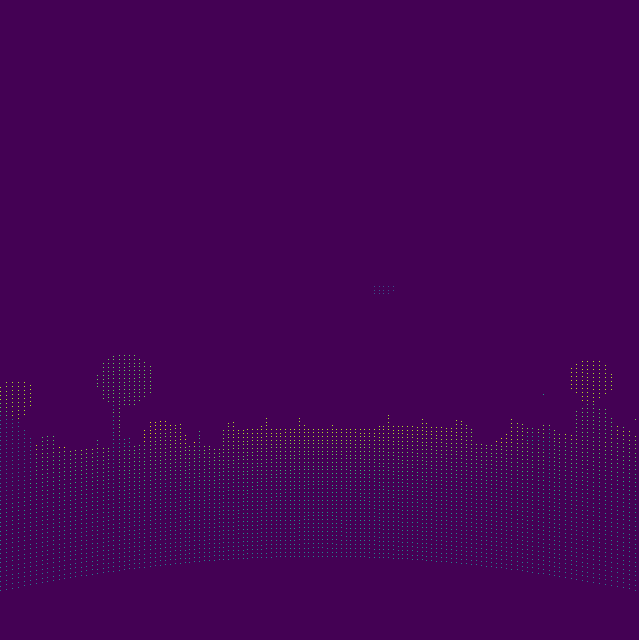
\includegraphics[width=\textwidth]{s2d_all.png}
		\caption{All pointcloud points.}
	\end{subfigure}
	\hfill
	\begin{subfigure}[b]{0.4\textwidth}
		\centering
		
\includegraphics[width=\textwidth]{s2d_select.png}
		\caption{Selected pointcloud points.}
	\end{subfigure}
	\caption{Sparse to dense training.}
\end{figure}
A processing algorithm was applied to the output depth map, further filtering points that were not in vicinity of the ground truth depth points. Both filtered and unfiltered depth maps were used for further training and testing to clarify their overall impact.
\begin{figure}[h!]
	\centering
	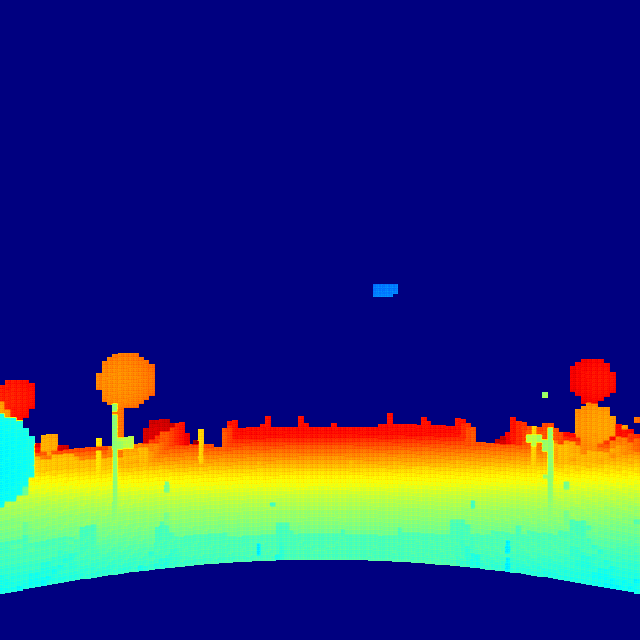
\includegraphics[width=5cm]{sparse2dense_filter.png}
	\caption{Applied filter on Sparse to dense output.}
\end{figure}
\section{Image inpainting}
An alternative algorithm for making sparse pointcloud into dense one was applied as well. The function is provided in OpenCV Python library. The input into the function was a sparse depth image, same as for the Sparse to dense network except the RGB part. The algorithm introduced in \ref{inpainting} was used with the radius of 1 pixel. The results were processed with the same filtering method as for the results of Sparse to dense method. For further training only the filtered depth map was used.
\begin{figure}[h]
	\centering
	\begin{subfigure}[b]{0.3\textwidth}
		\centering
		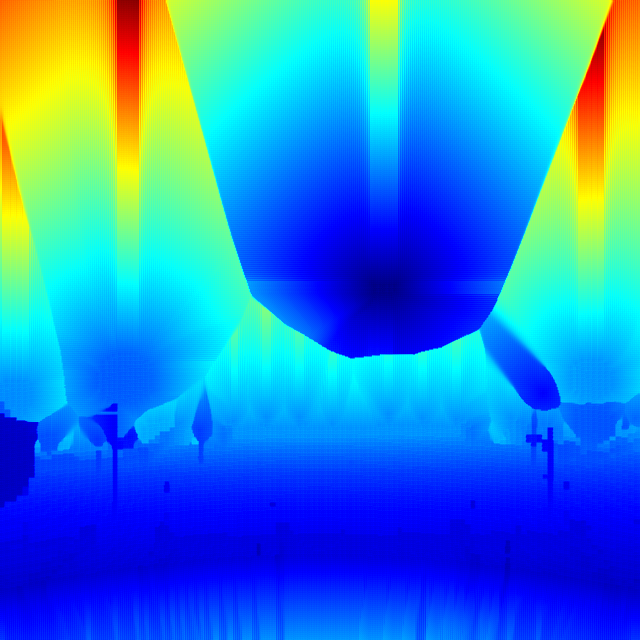
\includegraphics[width=\textwidth]{raw_inpaint.png}
		\caption{Non filtered result.}
	\end{subfigure}
	\hfill
	\begin{subfigure}[b]{0.3\textwidth}
		\centering
		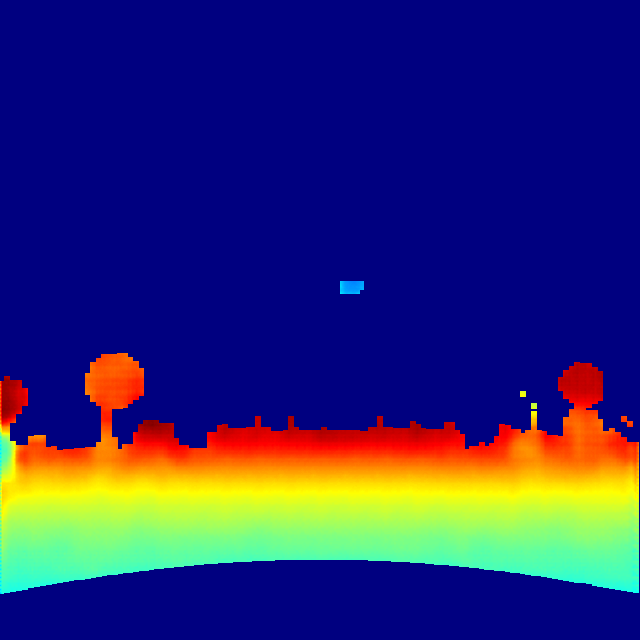
\includegraphics[width=\textwidth]{inpaint.png}
		\caption{Filtered result.}
	\end{subfigure}
	\caption{Inpaint results.}
\end{figure}
\section{YOLOv3}
Multiple different options of input to the YOLOv3 networks were applied. These include:
\begin{itemize}
	\item Concatenating the direct output of Sparse to dense neural network with the RGB images creating a RGBD image,
	\item Manually altering the dense depth image values that were inaccurate (f.e. sky) a changing them to a high value,
	\item Filtering the parts of the dense depth image that were very sparse in the original sparse depth image,
	\item Using OpenCV library to directly impaint the sparse depth image,
	\item Using only the RGB image skipping the depth entirely.
\end{itemize}
YOLOv3 PyTorch implementation was used for training. Further modifications were required to be made. The original implementation of YOLOv3 supports 3-channel RGB images as inputs. For the sake of this work a 4-channel RGB input option using H5 file system was implemented. The dataset consisted of drones of various sizes ranging from very small (few pixels) to very large closeups. Therefore 5 detection heads were implemented instead of the original 3. This ensured much higher detection confidence of smaller far away drones as well as bigger more close ones. The following parameters were used for training all inputs:
\begin{itemize}
	\item Number of epochs was set to 120,
	\item Batch size was set to 128,
	\item Size of the input images was 416x416x$n$, where $n\in\{3,4\}$,
	\item Learning rate was set to 0.001.
\end{itemize}
\begin{figure}[h]
	\centering
	\begin{subfigure}[b]{0.4\textwidth}
		\centering
		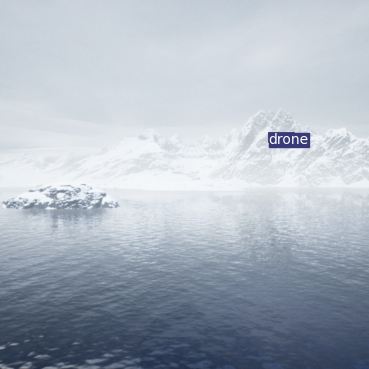
\includegraphics[width=\textwidth]{01640.png}
	\end{subfigure}
	\hfill
	\begin{subfigure}[b]{0.4\textwidth}
		\centering
		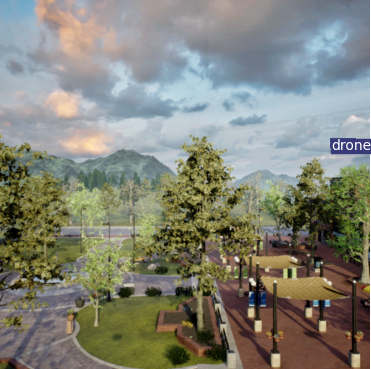
\includegraphics[width=\textwidth]{02002.png}
	\end{subfigure}
	\hfill
	\begin{subfigure}[b]{0.4\textwidth}
		\centering
		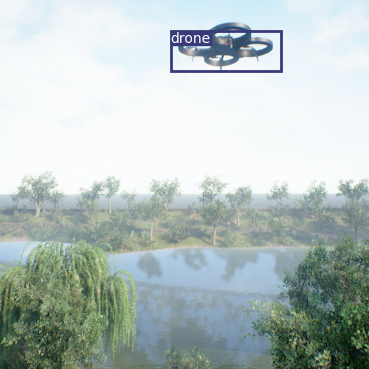
\includegraphics[width=\textwidth]{02167.png}
	\end{subfigure}
	\hfill
	\begin{subfigure}[b]{0.4\textwidth}
		\centering
		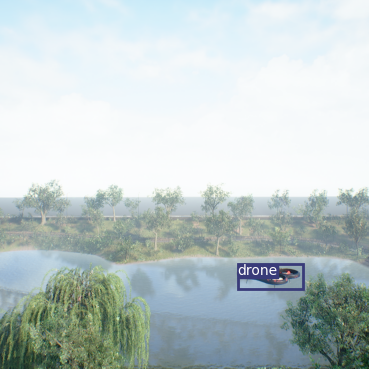
\includegraphics[width=\textwidth]{02665.png}
	\end{subfigure}
	\caption{Sample YOLOv3 outputs.}
\end{figure}
\chapter{Results}
After the training completed the different metrics on the validation dataset were compared. These metrics include:
\begin{itemize}
	\item Precision,
	\item Recall,
	\item Mean Average Precision (mAP).
\end{itemize}
These metrics are given by the following formulas:
\begin{equation}
\begin{aligned}
	Precision &= \frac{True Positives}{True Positives + False Positives}\\,
	Recall &= \frac{True Positives}{True Positives + False Negatives}\\,
	mAP &= \frac{1}{N}\sum^N_{i=1}AP_i,
\end{aligned}
\end{equation}
where:
\begin{itemize}
	\item $N$ is number of classes,
	\item $AP$ is Average Precision, an area under the Precision Recall curve.
\end{itemize}
For the RGBD dataset, where the depth map was taken as a direct output from trained Sparse to dense network a maximum mAP of 0.979 was achieved. For precision and recall, a maximum precision of 0.947 and a maximum recall of 0.991 were achieved.
\begin{figure}[h!]
	\centering
	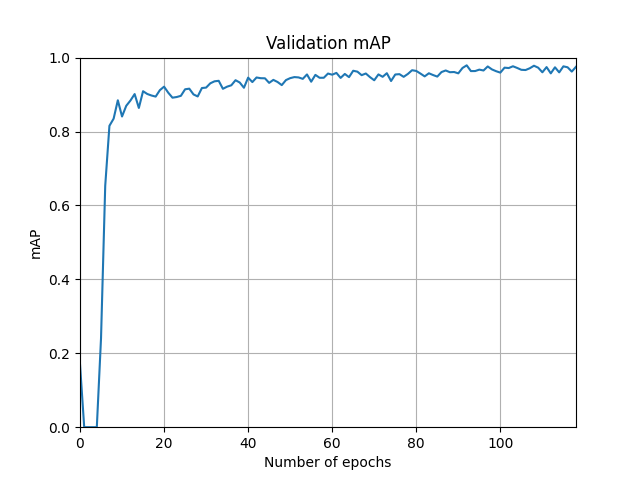
\includegraphics[width=\textwidth]{run-no_depth120e-tag-validation_mAP.png}
	\caption{mAP results of raw RGBD data.}
\end{figure}
\pagebreak
\begin{figure}[h!]
	\centering
	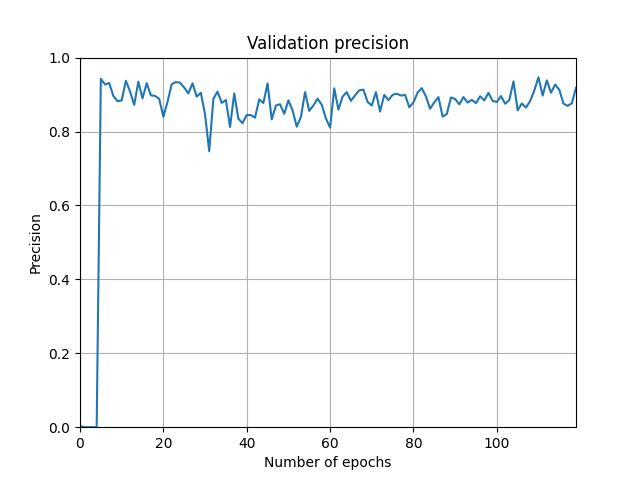
\includegraphics[width=\textwidth]{run-no_depth120e-tag-validation_precision.png}
	\caption{Precision results of raw RGBD data.}
\end{figure}
\begin{figure}[h!]
	\centering
	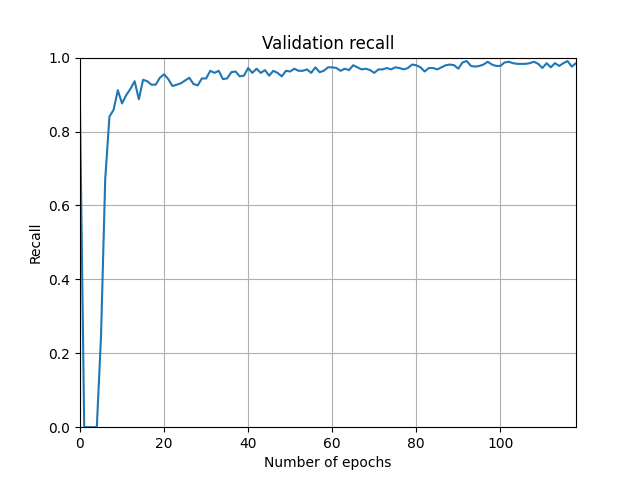
\includegraphics[width=\textwidth]{run-no_depth120e-tag-validation_recall.png}
	\caption{Recall results of raw RGBD data.}
\end{figure}
\pagebreak
\\
Next we look at the results of RGBD data from Sparse to dense network, where the depth map was manually altered. The maximum mAP was 0.971. The maximum Precision and Recall were 0.939 and 0.981 respectively.
\begin{figure}[h!]
	\centering
	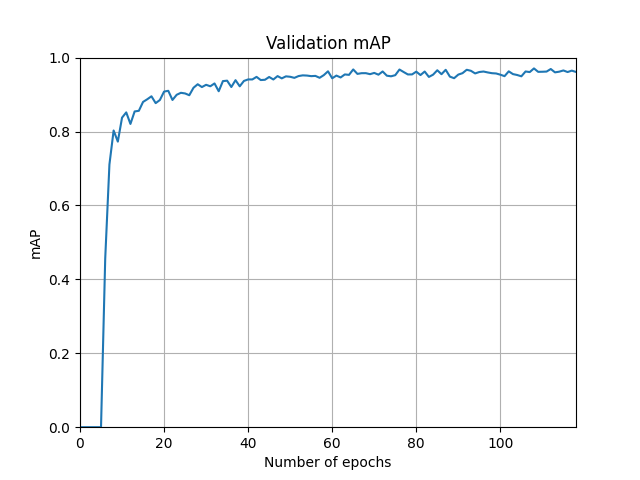
\includegraphics[width=\textwidth]{run-s2d_50filter-tag-validation_mAP.png}
	\caption{mAP results of manually altered RGBD data.}
\end{figure}
\pagebreak
\begin{figure}[h!]
	\centering
	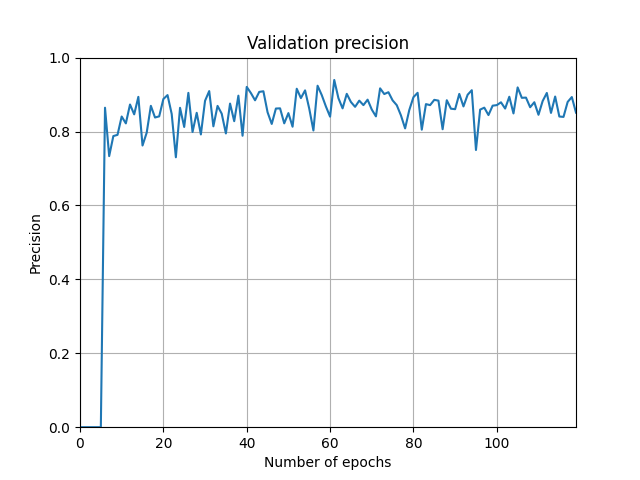
\includegraphics[width=\textwidth]{run-s2d_50filter-tag-validation_precision.png}
	\caption{Precision results of manually altered RGBD data.}
\end{figure}
\begin{figure}[h!]
	\centering
	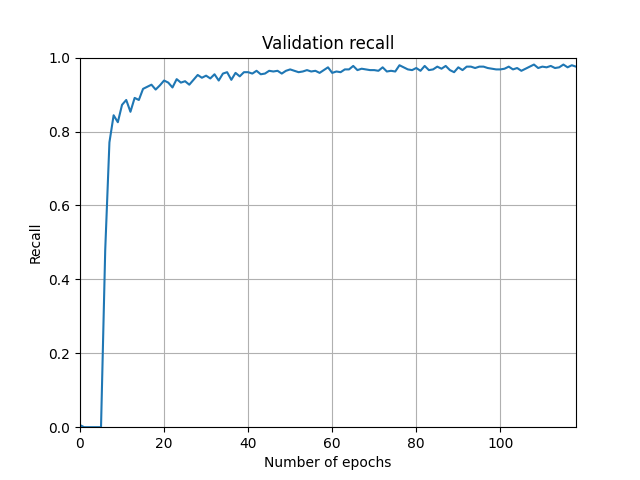
\includegraphics[width=\textwidth]{run-s2d_50filter-tag-validation_recall.png}
	\caption{Recall results of manually altered RGBD data.}
\end{figure}
\pagebreak
\\
For the RGBD data obtained from Sparse to dense network and altered based on the sparse depth map a maximum mAP of 0.948 was observed. The maximum Precision and Recall were both at 0.968.
\begin{figure}[h!]
	\centering
	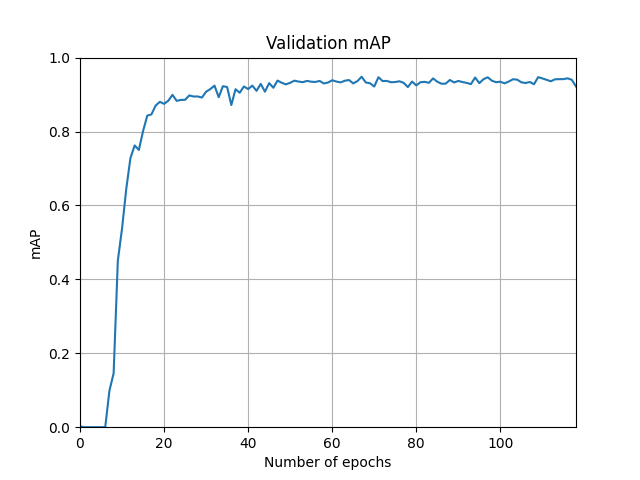
\includegraphics[width=\textwidth]{run-depth_filter120e-tag-validation_mAP.png}
	\caption{mAP results of altered RGBD data based on sparse depth map.}
\end{figure}
\pagebreak
\begin{figure}[h!]
	\centering
	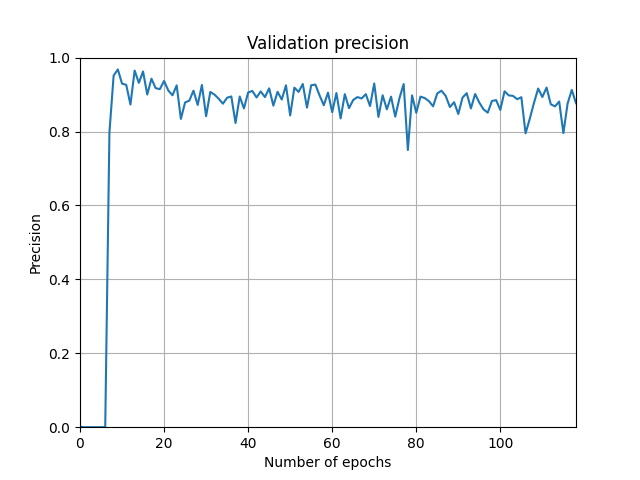
\includegraphics[width=\textwidth]{run-depth_filter120e-tag-validation_precision.png}
	\caption{Precision results of altered RGBD data based on sparse depth map.}
\end{figure}
\begin{figure}[h!]
	\centering
	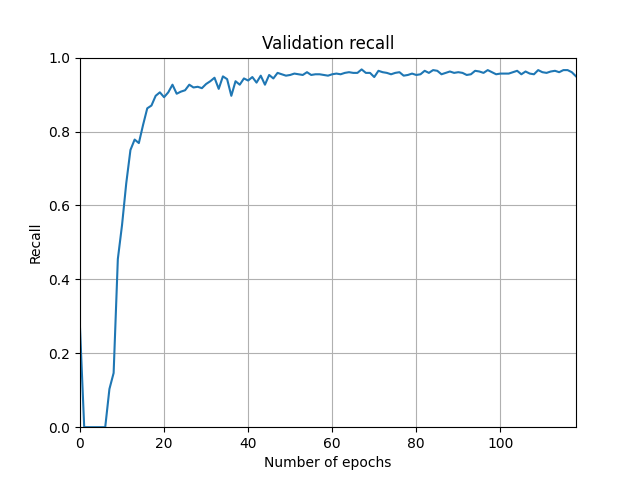
\includegraphics[width=\textwidth]{run-depth_filter120e-tag-validation_recall.png}
	\caption{Recall results of altered RGBD data based on sparse depth map.}
\end{figure}
\pagebreak
\\
Final RGBD dataset obtained by using the inpaint method resulted in maximum mAP of 0.979, maximum Precision of 0.969 and a maximum Recall of 0.99. 
\begin{figure}[h!]
	\centering
	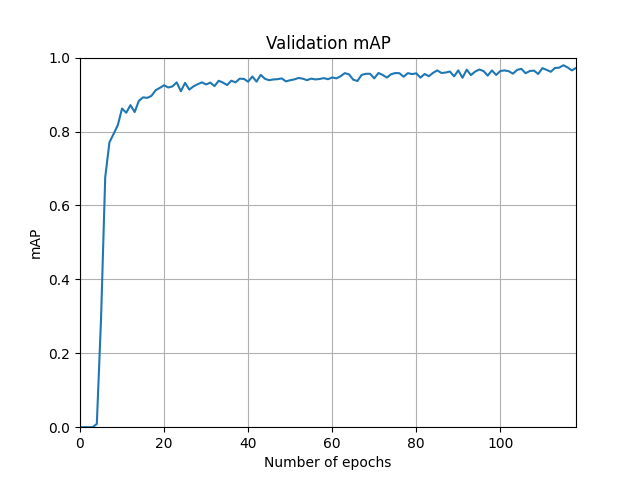
\includegraphics[width=\textwidth]{run-depth_inpaint-tag-validation_mAP.png}
	\caption{mAP results of RGBD data generated by inpaint method.}
\end{figure}
\pagebreak
\begin{figure}[h!]
	\centering
	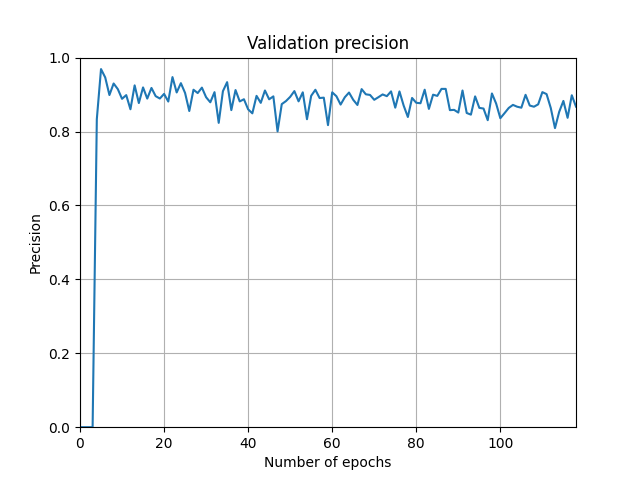
\includegraphics[width=\textwidth]{run-depth_inpaint-tag-validation_precision.png}
	\caption{Precision results of RGBD data generated by inpaint method.}
\end{figure}
\begin{figure}[h!]
	\centering
	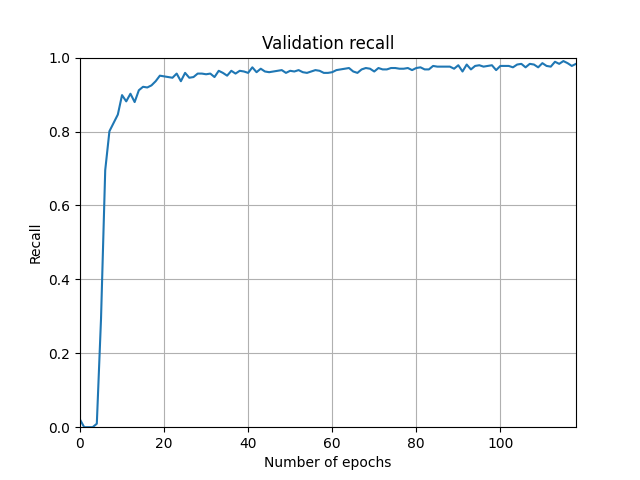
\includegraphics[width=\textwidth]{run-depth_inpaint-tag-validation_recall.png}
	\caption{Recall results of RGBD data generated by inpaint method.}
\end{figure}
\pagebreak
\\
For the RGB data a maximum mAP of 0.979, Precision of 0.947 and Recall of 0.99 was achieved.
\begin{figure}[h!]
	\centering
	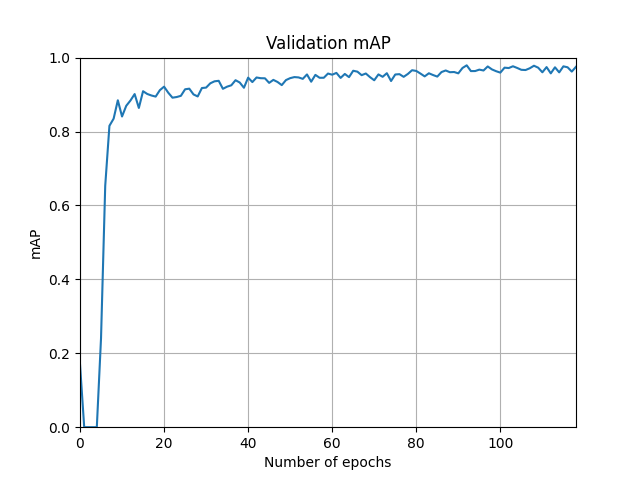
\includegraphics[width=\textwidth]{run-no_depth120e-tag-validation_mAP.png}
	\caption{mAP results of RGB data.}
\end{figure}
\pagebreak
\begin{figure}[h!]
	\centering
	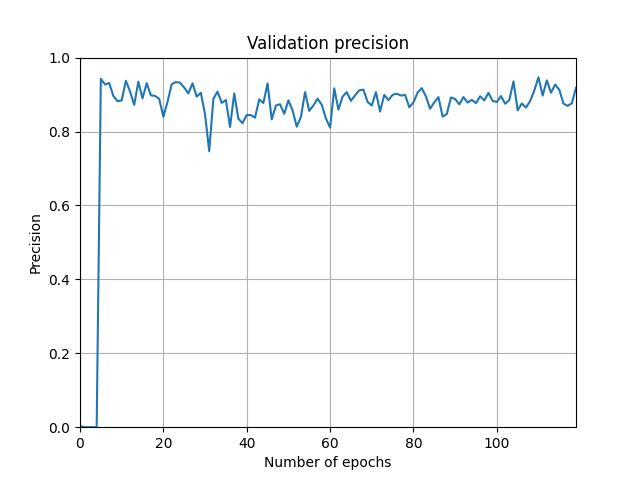
\includegraphics[width=\textwidth]{run-no_depth120e-tag-validation_precision.png}
	\caption{Precision results of RGB data.}
\end{figure}
\begin{figure}[h!]
	\centering
	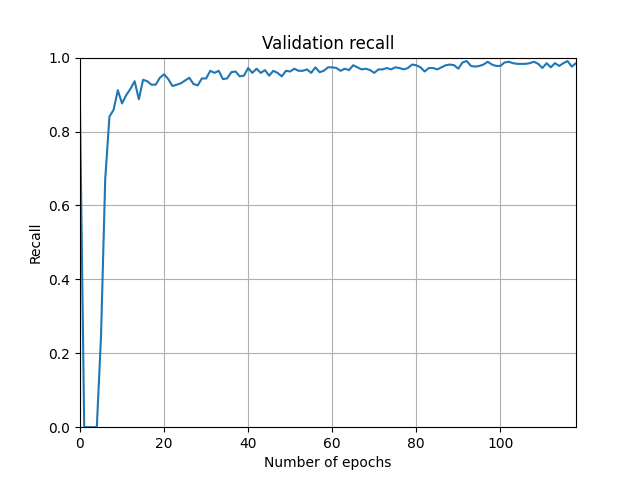
\includegraphics[width=\textwidth]{run-no_depth120e-tag-validation_recall.png}
	\caption{Recall results of RGB data.}
\end{figure}
\pagebreak
\\
Summarizing all the metrics from different methods a observation can be made. In terms of mAP and Recall the methods utilizing depth map provide no significant improvement over the pure RGB method. In terms of Precision a Inpaint RGBD and a Sparse depth map RGBD provide slight advantage and are better. In terms of Sparse to dense network output a dataset with sparse depth map that provides no information about significant portion of the picture offers only slight improvement in terms of Precision, but sacrificing mAP over RGB method after post-processing method applied.  
\begin{table}[h!]
	\centering
	\begin{tabular}{|c|c|c|c|c|c|}
		\hline
		Max       & Raw RGBD       & \begin{tabular}[c]{@{}c@{}}Manually altered \\ RGBD\end{tabular} & \begin{tabular}[c]{@{}c@{}}Sparse depth map \\ RGBD\end{tabular} & \begin{tabular}[c]{@{}c@{}}Inpaint \\ RGBD\end{tabular} & RGB            \\ \hline
		mAP       & \textbf{0.979} & 0.971                                                            & 0.948                                                            & \textbf{0.979}                                          & \textbf{0.979} \\ \hline
		Precision & 0.947          & 0.939                                                            & 0.968                                                            & \textbf{0.969}                                          & 0.947          \\ \hline
		Recall    & \textbf{0.991} & 0.981                                                            & 0.968                                                            & 0.99                                                    & 0.99           \\ \hline
	\end{tabular}
\caption{Summarized maximum values of different methods.}
\end{table}
\end{document}
